\subsection{Sprint 3}
\subsubsection{Sprint start}
This sprint was dedicated to work on the customers wishes for the application. A customer meeting had been done on the last day of last sprint. The meeting gave us a lot of good feedback about what to focus on.
What the team experienced had experienced previously was that it was hard to work on writing the application for the parts that was not well prototyped.
The decision thus, was to focus on having detailed, well thought prototypes, that would satisfy the customers feedback. 

For the parts of the application that we don't have time to implement, there will be a textual description.

\subsubsection{Sprint burndown}

The sprint burndown chart~\ref{fig:sprint3burndown} shows that progress was made a bit late, and that not enough time was spent.

\begin{figure}[H]
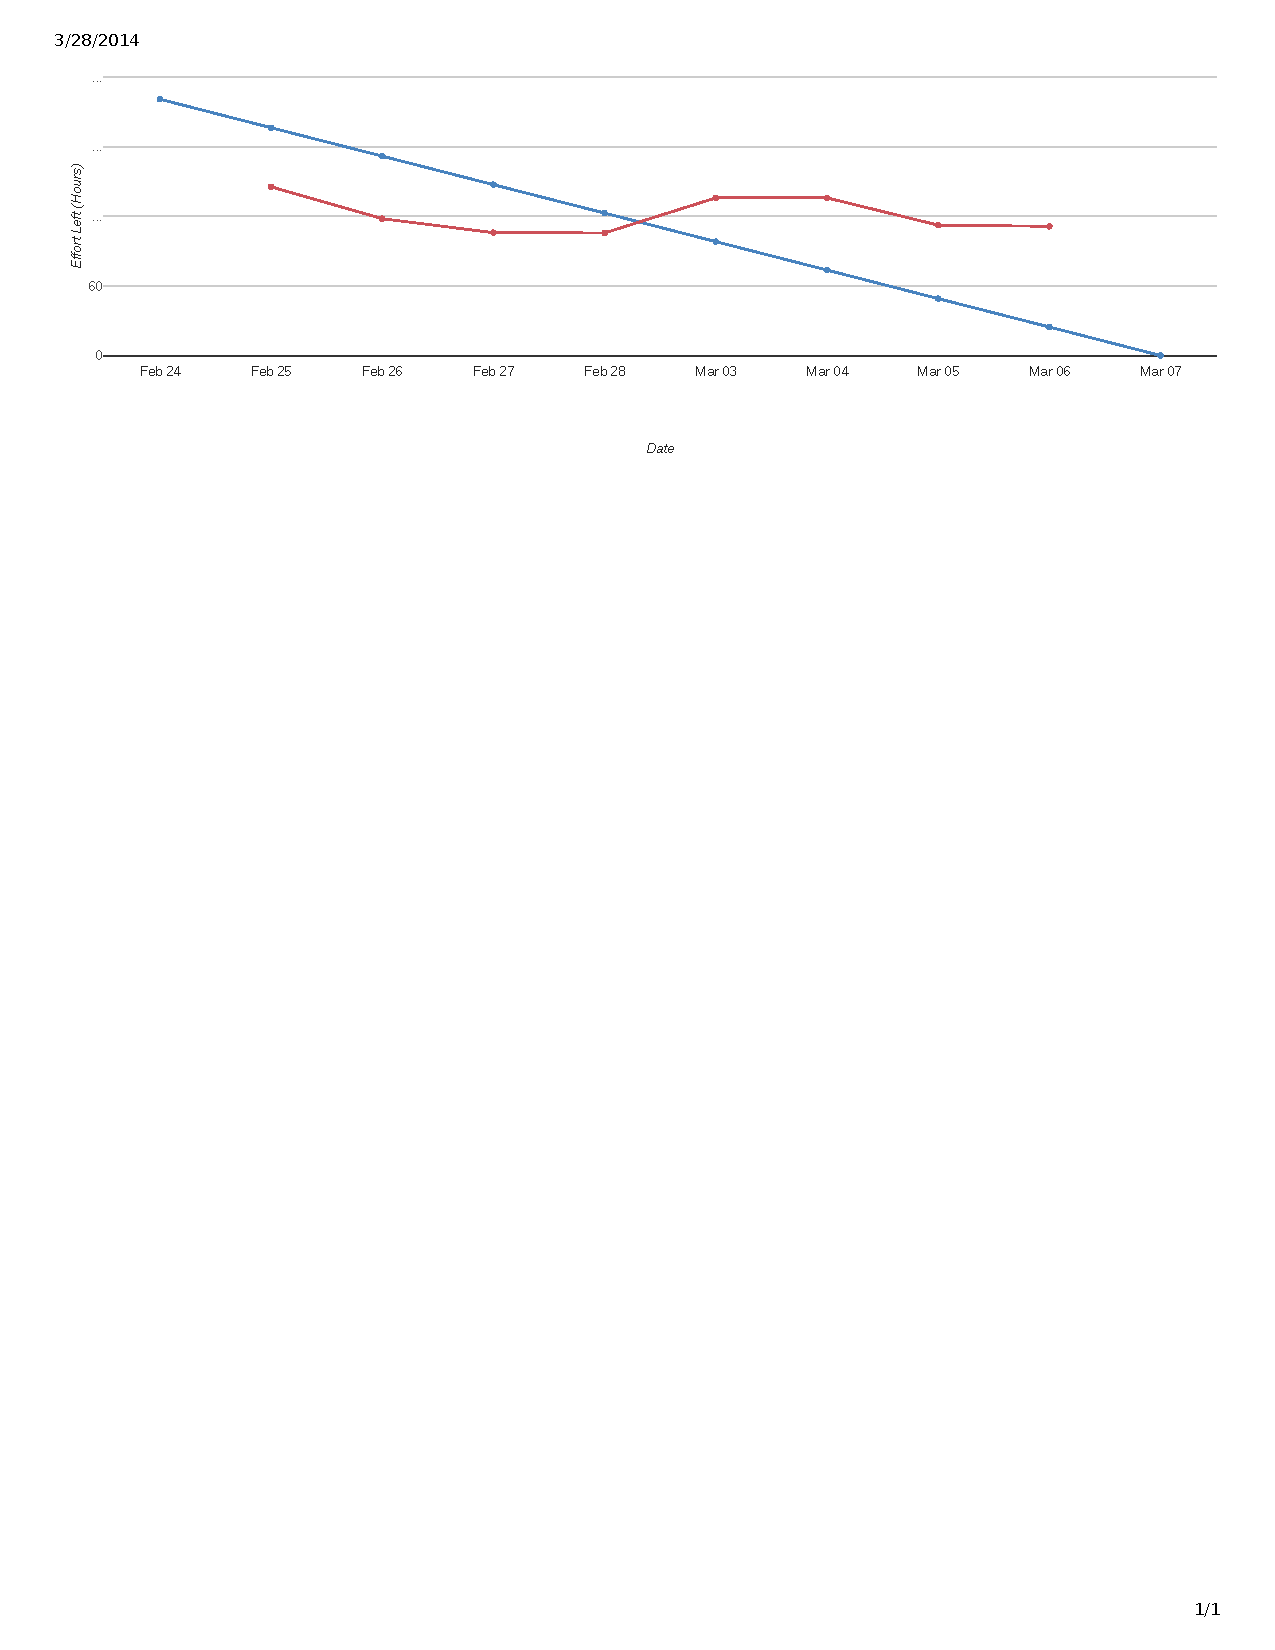
\includegraphics[width=\textwidth, trim= 1cm 21cm 1cm 1cm, clip=true]{ch/projectManagement/fig/burndown3.pdf}
\caption{Sprint 3 burndown chart}
\label{fig:sprint3burndown}
\end{figure}

\subsubsection{Sprint backlog}

The backlog and time usage result.

\begin{table}[H]
	\begin{tabular}{|l|p{7cm}|p{2.2cm}|p{1.5cm}|p{1.5cm}|}%
		\hline \bfseries User story & \bfseries Details & \bfseries Hours\newline estimated & \bfseries Hours spent & \bfseries Hours left
		\csvreader[head to column names]{ch/projectManagement/sec/sprints/sprint3/userstories.csv}{}% use head of csv as column names
		{\\\hline \id & \title & \estimated & \spent & \left} \\\hline% specify your coloumns here
	\end{tabular}
    \caption{Sprint 3 backlog}
\end{table}


\subsubsection{Sprint end}
After this sprint the application has detailed protypes for each part of the application. \todo[inline]{Må ha bilder av prototypene.} Some progress was also made on the actual implementation of the application.

There are two things to highlight in this sprint. The first is that the team has seen that much time is beeing spent discussing alot. The discussion are of importance, but it drains too much of the time the team members has. As to this, it has been decided that there should be set a certain about of time for the discussions. Should the discussions last longer than the time set, the project leader's task was to focus on ending the discussions, and instead perform a democratic vote based on the arguments that has been presented. 

Another issue is that not enough time was spent. During this sprint, some team  members have been sick. This was also a period where other subjects had big exercise deliveries. The key issue was that the needed effort for the other subjects was underestimated. As this is hard to forsee, the team can only but allocate more time to get back what was lost this sprint.